\documentclass[a4paper]{report}

\usepackage[a4paper]{geometry}
\usepackage{graphicx, amsmath, adjustbox, float}

% Title and Author Information
\title{CMPE 360 Fall 2023: Project 5 Report \\ Ray Tracing-2}
\author{Begüm Palaz \\ 17767049326}
\date{\today}

\geometry{
    a4paper,
    total={170mm,257mm},
    left=20mm,
    top=20mm,
}

\begin{document}

\maketitle

\section*{Introduction}
In this report for Project 5, we delve into the advanced aspects and applications of Ray Tracing-2, building upon the foundational principles covered earlier in the course to explore how this sophisticated rendering technique can enhance realism in computer graphics.

\section*{Checkpoint 4}

\textbf{Recursion and Reflection:} \\

When the depth is greater than zero, indicating that the ray can still be traced recursively, the direction of the reflected ray ($D_{\text{reflect}}$) is computed. This is calculated using the formula: \\
\begin{center}
    $D_{\text{reflect}} = \text{ray\_dir} - 2 \times (\text{ray\_dir} \cdot \text{hit\_norm}) \times \text{hit\_norm}$ \\
\end{center}

This reflects the incoming ray off the surface at an angle equal to the angle of incidence.
To avoid self-occlusion, the origin of the reflected ray ($\text{reflect\_orig}$) is slightly offset along the hit normal.
The reflected ray is then recursively traced by calling the  \texttt{RT\_trace\_ray} unction, and its color contribution ($L_{\text{reflect}}$) is computed.
Finally, this reflected light's contribution to the final color is added, scaled by the reflectivity ($k_r$) of the surface.

\begin{figure}[H]
    \begin{adjustbox}{lap=-1.5cm}
        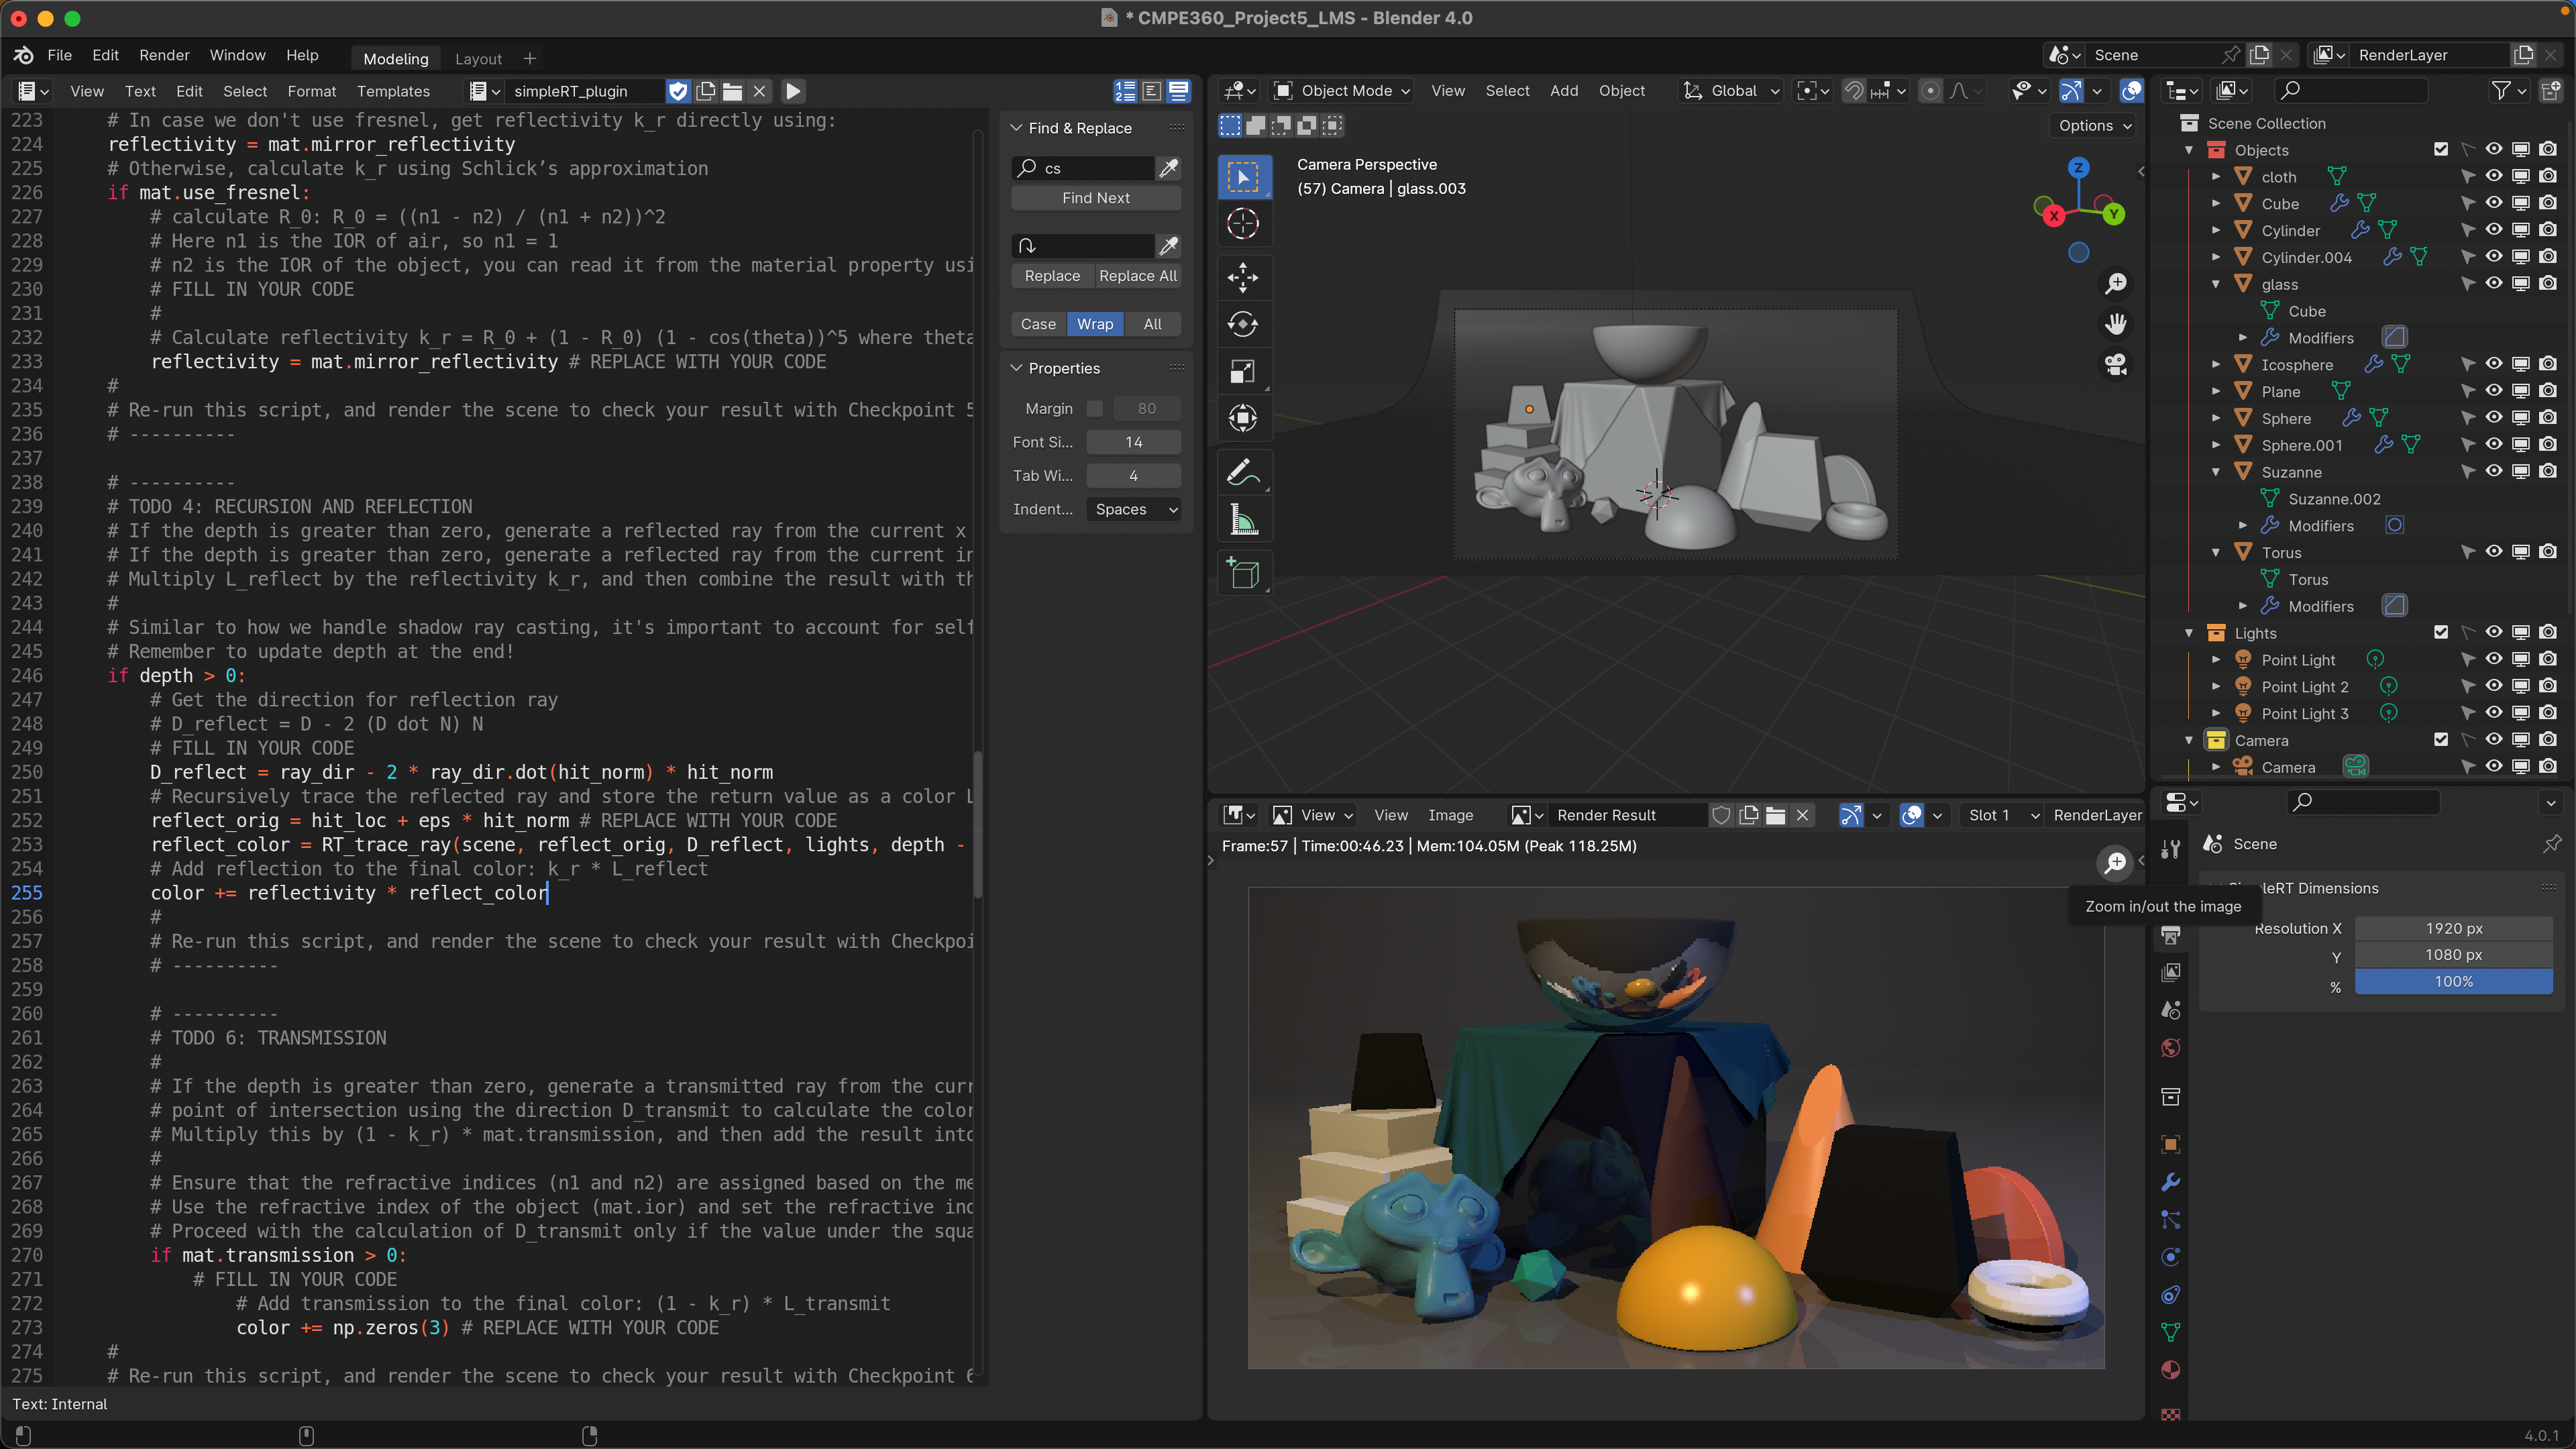
\includegraphics[width=1.2\textwidth]{chkpt4-ss.png}
    \end{adjustbox}
    \caption{Checkpoint 4: Reflections Screenshot}
    \label{fig:chkpt-ss}
\end{figure}

\begin{figure}[H]
    \begin{adjustbox}{lap=-1.5cm}
        \includegraphics[width=1.2\textwidth]{chkpt4.png}
    \end{adjustbox}
    \caption{Checkpoint 4: Reflections Output}
    \label{fig:chkpt4}
\end{figure}

\section*{Checkpoint 5}

\textbf{Fresnel Effect:} \\
The Fresnel effect calculates how reflectivity changes with the angle of incidence.
If Fresnel effect is not used, reflectivity ($k_r$) is directly taken as the mirror reflectivity of the material.
If Fresnel effect is used, Schlick's approximation is applied to calculate $k_r$.

\begin{center}
    $R_0 = \left(\frac{1 - \text{mat.ior}}{1 + \text{mat.ior}}\right)^2$
\end{center}

The Fresnel reflectivity ($k_r$) is then given by:
\begin{center}
    $k_r = R_0 + (1 - R_0) \times (1 - \cos(\theta))^5$
\end{center}

where $\theta$ is the angle of incidence, calculated using the dot product of the hit normal and the negative ray direction.

\begin{figure}[H]
    \begin{adjustbox}{lap=-1.5cm}
        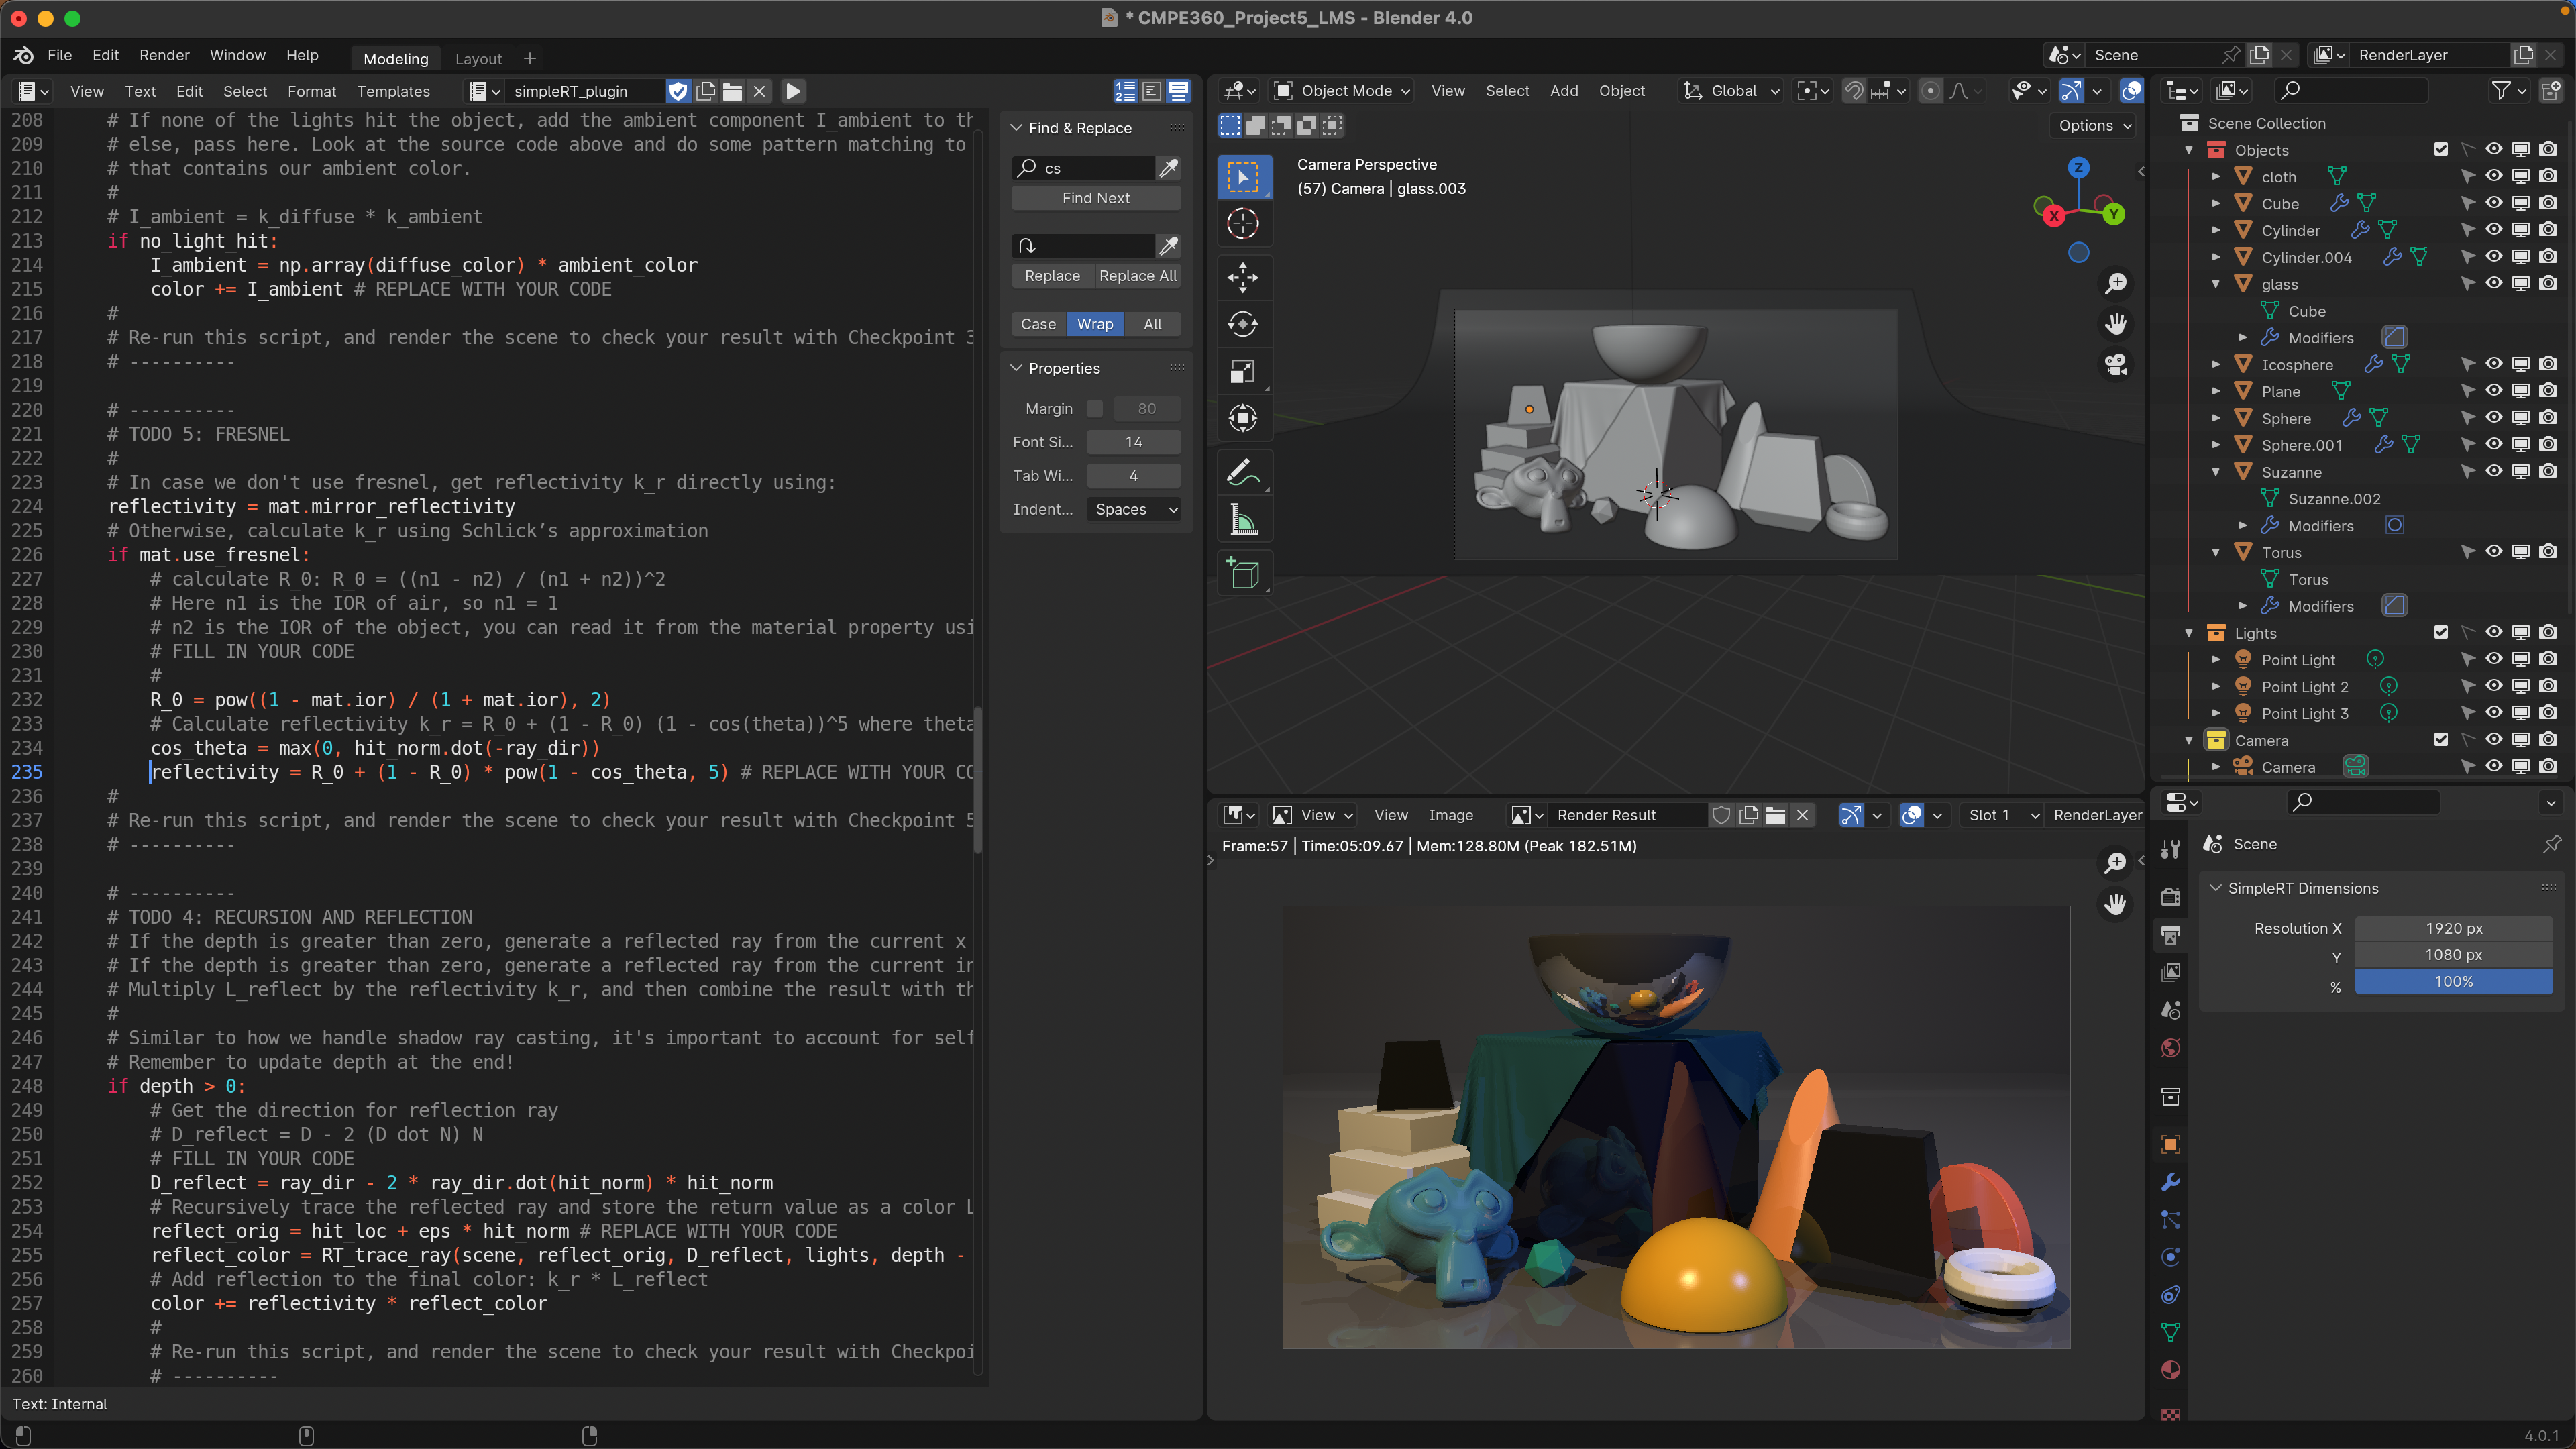
\includegraphics[width=1.2\textwidth]{chkpt5-ss.png}
    \end{adjustbox}
    \caption{Checkpoint 5: Fresnel Screenshot}
    \label{fig:chkpt5-ss}
\end{figure}

\begin{figure}[H]
    \begin{adjustbox}{lap=-1.5cm}
        \includegraphics[width=1.2\textwidth]{chkpt5.png}
    \end{adjustbox}
    \caption{Checkpoint 5: Fresnel Output}
    \label{fig:chkpt5}
\end{figure}

\section*{Checkpoint 6}

\textbf{Transmission:} \\
This part handles the transmission (or refraction) of the ray through a transparent material. Based on Snell's law, the refractive indices of air ($n1$) and the material ($n2$) are used. 
If the ray is inside the object, $n1$ and $n2$ are swapped. 
The ratio of these indices ($\eta$) is calculated, and the sine of the transmitted angle squared ($\sin^2(t)$) is derived from it. 
If there's no total internal reflection (checked using $\sin^2(t) < 1$), the direction for the transmitted ray ($D_{\text{transmit}}$) is calculated. 
The origin for the transmission ray is offset to avoid self-occlusion. 
The transmitted ray is then recursively traced, and its color contribution ($L_{\text{transmit}}$) is added to the final color, weighted by $(1 - k_r)$.

\begin{figure}[H]
    \begin{adjustbox}{lap=-1.5cm}
        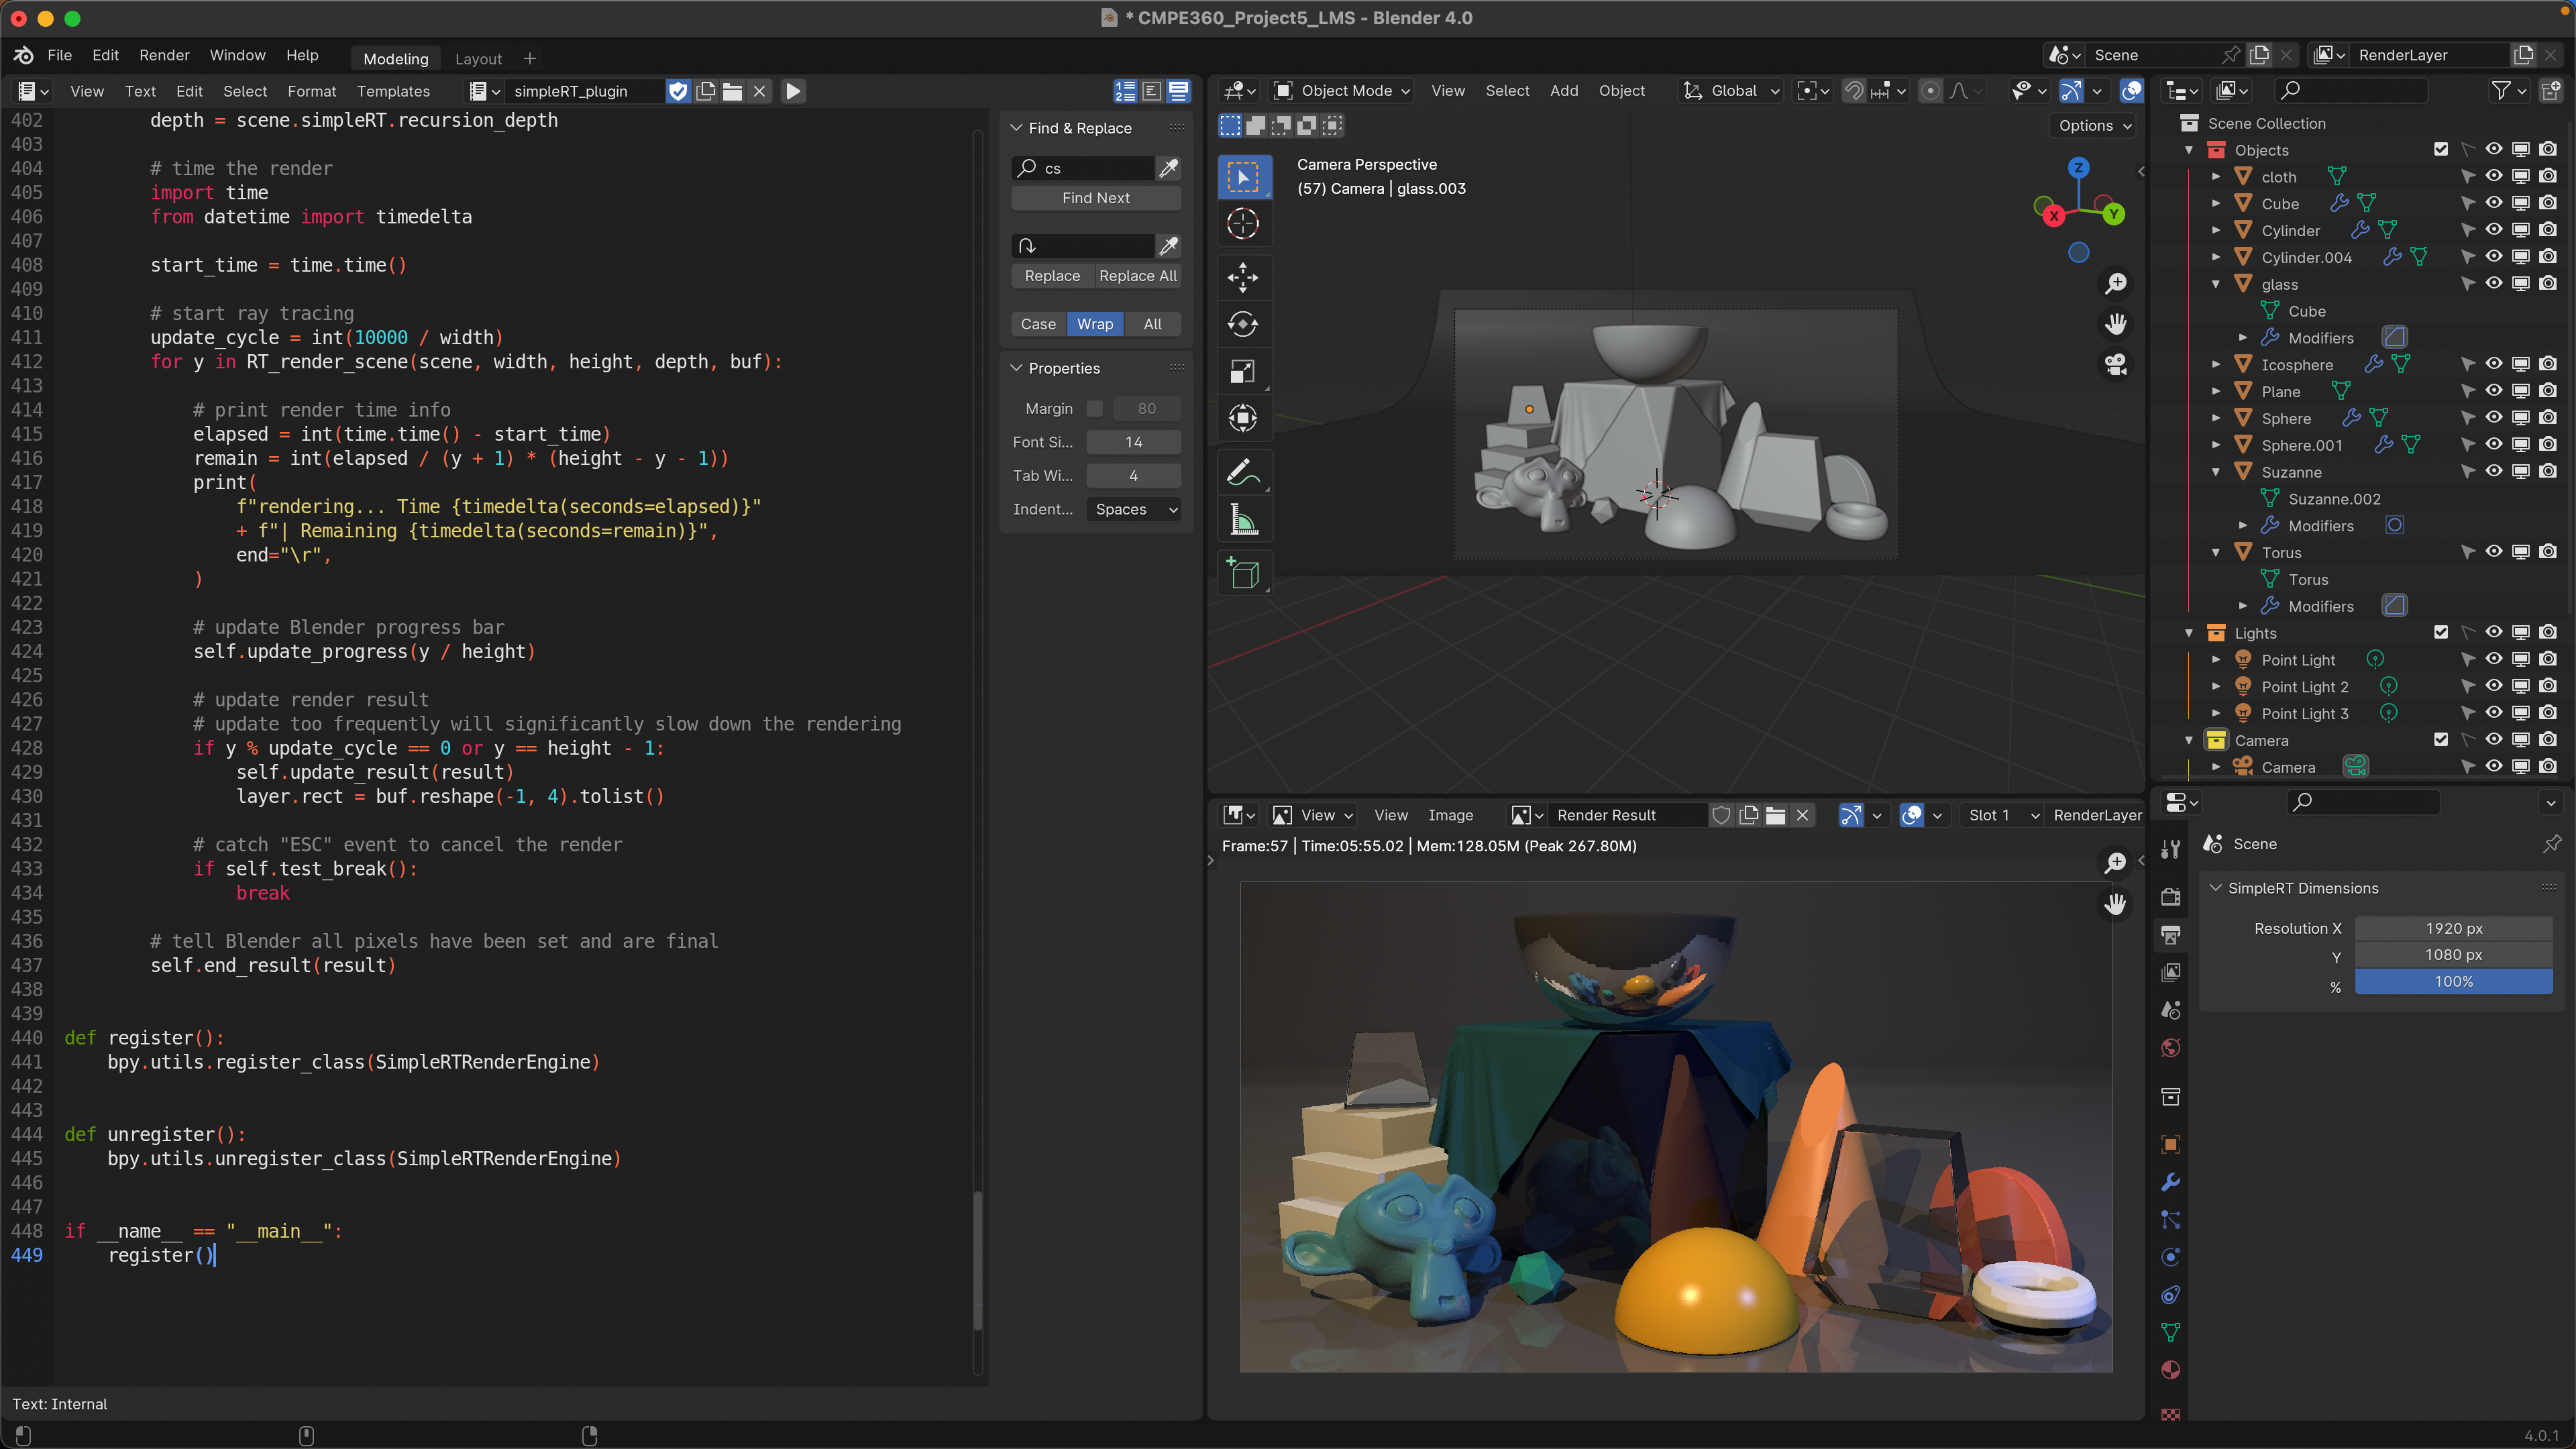
\includegraphics[width=1.2\textwidth]{chkpt6-ss.png}
    \end{adjustbox}
    \caption{Checkpoint 6: Transmission Screenshot}
    \label{fig:chkpt6-ss}
\end{figure}

\begin{figure}[H]
    \begin{adjustbox}{lap=-1.5cm}
        \includegraphics[width=1.2\textwidth]{chkpt6.png}
    \end{adjustbox}
    \caption{Checkpoint 6: Transmission Output}
    \label{fig:chkpt6}
\end{figure}

\end{document}